\section{Missing Proofs and Details of Section~\ref{sec:geo-primal-dual}}\label{sec:appendix-geo-primal-dual}
In this section, we first present a sweep-line algorithm for constructing the hierarchical partitioning described in Section~\ref{sec:hierarchical}. We then present the missing proofs of lemmas in Sections~\ref{sec:geo-primal-dual}.


\myparagraph{Constructing the hierarchical partitioning.} Recall that, as described in Section~\ref{sec:hierarchical}, our algorithm constructs a hierarchical partitioning by recursively partitioning each non-leaf cell of $\mcH$ into two smaller cells as its children. We describe the partitioning procedure with respect to an arbitrary cell $\cell$ of $\mcH$. Let $\ell_x$ and $\ell_y$ denote the width and length of $\cell$, and without loss of generality, assume $\ell_x\ge \ell_y$. Let $x_{\min}$ (resp. $x_{\max}$) denote the $x$ coordinate of the left (resp. right) side of $\cell$. Recall that $\lambda=9n^{-1/5}$. Define a priority queue $\mcQ$ storing two events for each point $u\in A_\cell\cup B_\cell$, namely an entry event $e_u^\downarrow$ at $u_x-\ell_\cell\lambda$ and an exit event $e_u^\uparrow$ at $u_x + \ell_\cell\lambda$; here, $u_x$ denotes the $x$ coordinate of point $u$. See the events $b^\downarrow$ and $b^\uparrow$ in Figure~\ref{fig:sweepline}.

Consider a vertical sweep line that moves from left to right, searching for a value $x^* \in [x_{\min} + \frac{\ell_x}{3}, x_{\min} + \frac{2\ell_x}{3}]$ that minimizes $|\Lambda(x^*)|$; recall that $\Lambda(x):=\{u\in A_\cell\cup B_\cell: |u_x-x|\le \ell_\cell\lambda\}$ for any $x\in [x_{\min} + \frac{\ell_x}{3}, x_{\min} + \frac{2\ell_x}{3}]$. Let $x'$ denote the state of the sweep line. Intuitively, as the sweep line moves from left to right (i.e., $x'$ increases), any point $u\in A_\cell\cup B_\cell$ enters the set $\Lambda(x')$ at its entry event and exits $\Lambda(x')$ at its exit event. Thus, we can keep track of the number of points close to the sweep line by incrementing (resp. decrementing) the count at each entry (resp. exit) event and return the value $x^*$ realizing the minimum count during the sweep-line procedure. 

More formally, we maintain a value $\gamma$ representing the number of points of $A_\cell\cup B_\cell$ at a distance at most $\ell_\cell\lambda$ to the sweep line. We also store, for a set of $O(n_\cell)$ values $x''\in [x_{\min}, x_{\max}]$, a function $\eta:[x_{\min}, x_{\max}] \rightarrow \mbZ_{\ge 0}$ representing $|\Lambda(x'')|$. Initially, for the minimum event $e$ in $\mcQ$, set $\gamma\leftarrow 1$ and $\eta(e)\leftarrow \gamma$. Iteratively, our sweep-line algorithm extracts the minimum event $e$ from $\mcQ$. If $e$ is an entry event, set $\gamma\leftarrow \gamma + 1$, and otherwise, $e$ is an exit event and set $\gamma\leftarrow \gamma - 1$. Set $\eta(e)\leftarrow \gamma$. After processing all events in $\mcQ$, define the entry $x'$ of $\eta(\cdot)$ in the middle third of $x$ side of $\cell$ with the minimum value, i.e., \[x^*:=\arg\min_{x\in [x_{\min}+\frac{\ell_\cell}{3}, x_{\min}+\frac{2\ell_\cell}{3}]\cap S(\eta)}\eta(x),\] where $S(\eta)$ denotes the support of $\eta$. Partition $\cell$ using the vertical line $x=x^*$ into two smaller cells $\cell_1$ and $\cell_2$, and add the non-empty ones as the children of $\cell$ to $\mcH$. 
\begin{figure}
    \centering
    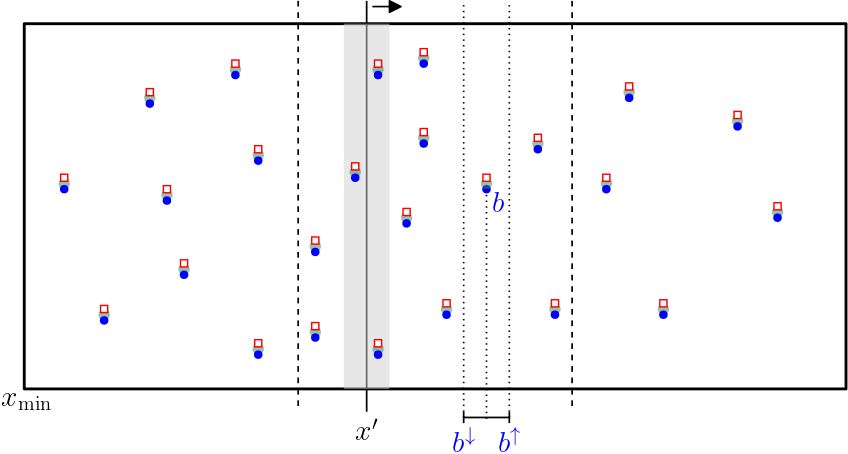
\includegraphics[width=0.7\linewidth]{figures/sweepline.png}
    \caption{The solid vertical line shows the line our sweep-line procedure maintains. The two values $b^\downarrow$ and $b^\uparrow$ show the entry and exit events created for the blue point $b$.}
    \label{fig:sweepline}
\end{figure}





\subsection{Missing Proofs of Section~\ref{sec:geo-primal-dual}}

\margin*
\begin{proof}
    We use an inductive proof to show that the aspect ratio of all cells of $\mcH$ is at most $3$. Note that the root cell $\cell^*$ is square and has a unit aspect ratio. For any non-root cell $\cell\in \mcH$, let $\cell'$ denote the parent of $\cell$ in $\mcH$. By the inductive hypothesis, the aspect ratio of $\cell'$ is at most $3$. Let $\ell_x$ (resp. $\ell_y$) denote the width (resp. length) of $\cell$. Similarly, let $\ell'_x$ (resp. $\ell'_y$) denote the width (resp. length) of $\cell'$. Without loss of generality, assume $\ell'_x\ge \ell'_y$. In this case, we split $\cell'$ into two rectangles using a vertical line in the middle third part of the $x$ side of $\cell'$, i.e., $\ell_y=\ell'_y$ and $\ell_x\in [\frac{\ell'_x}{3}, \frac{2\ell'_x}{3}]$. In this case, if $\ell_x\ge \ell_y$, then $\frac{\ell_x}{\ell_y}\le \frac{\ell'_x}{\ell'_y}\le 3$. Otherwise, $\ell_x< \ell_y$ and $\frac{\ell_y}{\ell_x}\le \frac{\ell'_y}{\ell'_x/3}\le 3$.

    Next, we show that the number of points of $A_\cell\cup B_\cell$ at a distance at most $\ell_\cell\lambda$ from the divider $\divider\cell$ is $O(n_\cell \lambda)$. Consider the set $\zeta=\{x_{\min}+\frac{\ell_\cell}{3} + 3i \ell_\cell\lambda: 0\le i\le \lfloor \frac{1}{9\lambda}\rfloor\}$. Recall that for any value $x'\in[x_{\min}+\frac{\ell_\cell}{3}, x_{\min}+\frac{2\ell_\cell}{3}]$, $\Lambda(x')$ denotes the set of all points of $A_\cell\cup B_\cell$ that are at a distance at most $\ell_\cell\lambda$ from the vertical line $x=x'$. 
    Note that for any pair of distinct values $x_1, x_2\in \zeta$, $\Lambda(x_1)\cap\Lambda(x_2)=\emptyset$. See Figure~\ref{fig:sweepline2}. 
    \begin{figure}
        \centering
        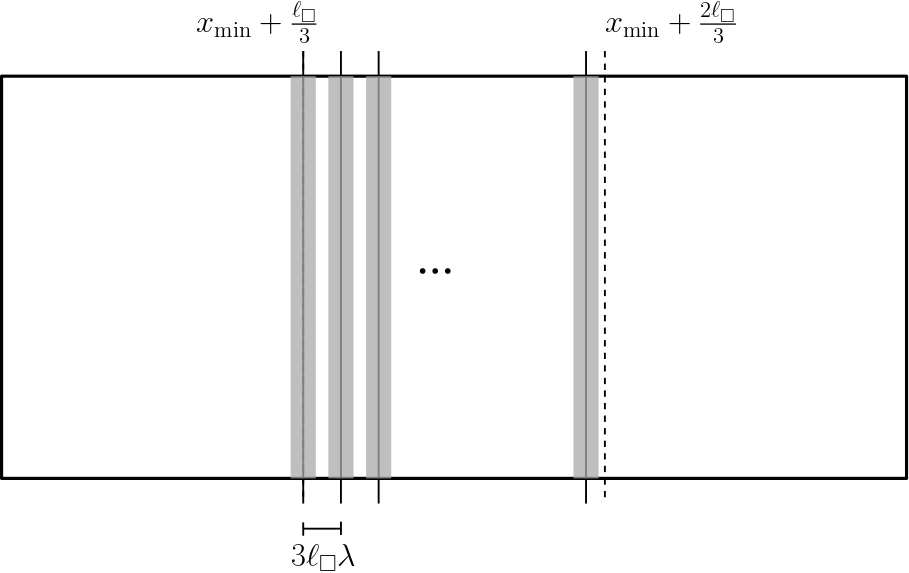
\includegraphics[width=0.9\linewidth]{figures/sweepline2.png}
        \caption{The solid vertical line shows the set $\zeta$.}
        \label{fig:sweepline2}
    \end{figure}
    Furthermore, 
    \[
    \sum_{x'\in \zeta} |\Lambda(x')| \le n_\cell.\]
    Define $x^*:=\arg\min_{x'\in\zeta}|\Lambda(x')|$. In this case, the size of $\Lambda(x^*)$ is no more than the average size of the $\Lambda(x')$ for the values $x'\in \zeta$; more precisely,
    \[|\Lambda(x^*)| \le \frac{\sum_{x'\in \zeta} |\Lambda(x')|}{|\zeta|} \le 9\lambda n_\cell. \]
\end{proof}

\geometricAnalysis*
\begin{proof}
    Define $\mbG$ to be a grid of cell-side-length $\ell_\cell n_\cell^{-2/5}$ that partitions $\cell$ into $O(n_\cell^{4/5})$ equal-sized rectangles. For each rectangle $\xi$ of the grid $\mbG$, let $\requests_\xi=\langle r'_1, \ldots, r'_m\rangle$ denote the sub-sequence of requests in $\requests$ that lie inside $\xi$, and let $A_\xi$ (resp. $B_\xi$) denote the subset of $A_\cell$ (resp. $B_\cell$) that lie inside $\xi$. Define $\mcG_\xi$ as the sub-graph of $\mcG$ induced by $A_\xi\cup B_\xi$. Let $M_\xi$ denote the set of edge $(a_{r'_i}, b_{r'_{i+1}})$ for all $i\in[1, m-1]$. $M_\xi$ is a matching on $\mcG_\xi$ that matches all except one point of $B_\xi$. Furthermore, since each matching edge in $M_\xi$ has a cost at most $2\ell_\cell n_\cell^{-2/5}$, the cost of $M_\xi$ would be $O(\ell_\cell |B_\xi| n_\cell^{-2/5})$.

    \begin{figure}
        \centering
        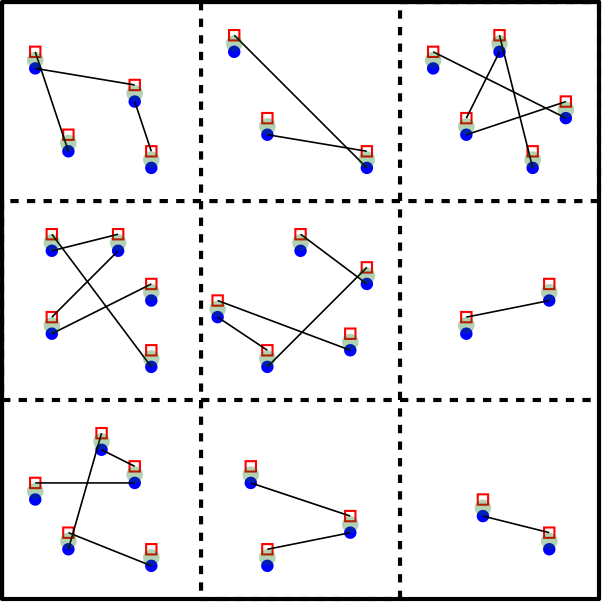
\includegraphics[width=0.5\linewidth]{figures/geo.png}
        \caption{A matching $M_\xi$ is computed inside each square $\xi$ by connecting the requests in their arrival order.}
        \label{fig:geo}
    \end{figure}
    
    Define $M':=\bigcup_{\xi\in\mbG}M_\xi$ as the union of the matchings computed inside each cell of the grid $\mbG$. Since $|\mbG|=O(n_\cell^{4/5})$ and each cell leaves at most one point of $B_\cell$ unmatched, the matching $M'$ matches all except $O(n_\cell^{4/5})$ points of $B_\cell$. In addition, the cost of $M$ is at most \[w(M')=\sum_{\xi\in\mbG}w(M_\xi)=O\left(\ell_\cell n_\cell^{-2/5}\sum_{\xi\in\mbG}|B_\xi|\right) = O(\ell_\cell n_\cell^{3/5}).\]
\end{proof}

We next present a set of definitions, which are used in the proof of Lemma~\ref{lemma:root-inactive}. Given a matching $M$ on the graph $\mcG_\sigma$, any simple path $P$ is an alternating path if the edges of $P$ alternate between matching and non-matching edges with respect to $M$. The path $P$ is called a (standard) augmenting path if it starts from an unmatched point $b\in B$ and ends at an unmatched point $a\in A$. One can augment $M$ along $P$ by setting $M\leftarrow M\oplus P$. The net-cost of $P$ is defined as $\phi(P):=\sum_{(a,b)\in P\setminus M}d(a,b) - \sum_{(a,b)\in P\cap M}d(a,b)$, i.e., the net-cost of $P$ is the change in the matching cost introduced by augmenting $M$ along $P$.

\rootinactive*
\begin{proof}
    For the sake of contradiction, suppose the matching $M$ is not a $t$-matching, and there exist boundary-matched points in $B^{\mcC^*}$. To prove this lemma, we show that there exists an extended matching $\hat{M}^{\mcC^*}=(\hat{M}, \hat{B}^{\mcC^*})$ of size $t$ such that $|\hat{M}|>|M|$ and $w_{\mcC^*}(\hat{M}^{\mcC^*})<w_{\mcC^*}(M^{\mcC^*})$, contradicting the assumption that $M^{\mcC^*}$ is a minimum-cost extended $t$-matching. 

    Consider a minimum net-cost augmenting path $P$ with respect to the matching $M$ from an unmatched point $b\in B$. Since the path $P$ has a length of at most $2n-1$, the net-cost of $P$ is 
    \begin{align*}
        \phi(P) = \sum_{(a,b)\in P\setminus M}d(a,b) - \sum_{(a,b)\in P\cap M}d(a,b) \le \sum_{(a,b)\in P\setminus M}d(a,b) \le 2n,  
    \end{align*}
    where the last inequality holds since all points are in the unit square and the $\ell_p$ distance of each pair is at most $2$. By augmenting the matching $M$ along the path $P$, we get a matching $\hat{M}$ with a cost $w(\hat{M})=w(M)+\phi(P)\le w(M) + 2n$. Also note that by the construction of $\cell^*$, for any point $b'\in B$, $\distance{b'}{\cell^*}\ge 3n-1$. If the endpoint $b$ of $P$ is in $B^{\mcC^*}$, then for the extended matching $\hat{M}^{\mcC^*}=(\hat{M}, B^{\mcC^*}\setminus\{b\})$, 
    \begin{align*}
        w_{\mcC^*}(\hat{M}^{\mcC^*})&= w(\hat{M}) + \sum_{b'\in B^{\mcC^*}\setminus\{b\} }\distance{b'}{\mcC^*}
        \le w(M) + 2n + \sum_{b'\in B^{\mcC^*}\setminus\{b\} }\distance{b'}{\mcC^*}\\&<w(M) + \distance{b}{\mcC^*} + \sum_{b'\in B^{\mcC^*}\setminus\{b\}}\distance{b'}{\mcC^*}=
        w_{\mcC^*}(M^{\mcC^*}).
    \end{align*}
    Otherwise, let $\hat{b}\in B^{\mcC^*}$ denote an arbitrary boundary-matching point of $M^{\mcC^*}$. Then, for the extended matching $\hat{M}^{\mcC^*}=(\hat{M}, B^{\mcC^*}\setminus\{\hat{b}\})$, 
    \begin{align*}
        w_{\mcC^*}(\hat{M}^{\mcC^*})&= w(\hat{M}) + \sum_{b'\in B^{\mcC^*}\setminus\{\hat{b}\} }\distance{b'}{\mcC^*}
        \le w(M) + 2n + \sum_{b'\in B^{\mcC^*}\setminus\{\hat{b}\} }\distance{b'}{\mcC^*}\\&<w(M) + \distance{\hat{b}}{\mcC^*} + \sum_{b'\in B^{\mcC^*}\setminus\{\hat{b}\}}\distance{b'}{\mcC^*}=
        w_{\mcC^*}(M^{\mcC^*}).
    \end{align*}
    Note that in both cases, $\hat{M}^{\mcC^*}$ is also of size $t$, which is a contradiction to the assumption that $M^{\mcC^*}$ is a minimum-cost extended $t$-matching. Therefore, the extended matching $M^{\mcC^*}=(M, B^{\mcC^*})$ has no boundary-matched points and $|M| = t$. 
    Consequently, $w_{\mcC^*}(M^{\mcC^*}) = w(M)$, and since $M^{\mcC^*}$ has the minimum cost among all extended $t$-matchings, the matching $M$ would have a minimum cost among all $t$-matchings on $\mcG_\sigma$, i.e., $M$ is a minimum-cost $t$-matching.
\end{proof}
% \begin{proof}
%     By the definition of the $\cell^*$-optimality, the matching $M, y(\cdot)$ is a $\cell^*$-feasible on $\mcG_\requests$, has a total of $t$ matched and inactive free vertices of $B$, and satisfies the condition (C1). First, note that if $t=n-1$, then the matching $M$ is the unique matching corresponding to the unique $1$-partitioning of the requests in $\requests$ and therefore, is the minimum-cost $t$-matching. Hence, in the following of this proof, we assume that $t<n-1$.
    
%     By Lemma~\ref{lemma:no-map-boundary}, the matching $M, y(\cdot)$ contains no inactive free points of $B$, and therefore, all free points with respect to $M, y(\cdot)$ are active. Define $y_{\max}:=\max_{b'\in B}y(b')$. Let $A_F$ (resp. $B_F$) denote the set of free points of $A$ (resp. $B$). By condition (C1), for any free point $b\in B_F$, $y(b)=y_{\max}$ and for any free point $a\in A_F$, $y(a)=0$.  Using the feasibility condition~\eqref{eq:dualfeasibility-matching-time}, we can rewrite the cost of the matching $M$ as
%     \begin{align}
%         w(M) &= \sum_{(a,b)\in M} \distance{a}{b} = \sum_{(a,b)\in M} y(b) - y(a)\nonumber \\ &= \left(\sum_{b\in B} y(b) - \sum_{a\in A} y(a)\right) - \sum_{b\in B_F} y(b) + \sum_{a\in A_F} y(a)\nonumber \\ &= \left(\sum_{b\in B} y(b) - \sum_{a\in A} y(a)\right) - |B_F|\cdot y_{\max}.
%         \label{eq:dualOptimal-proof-1}
%     \end{align}
%     Let $M^*$ denote any minimum-cost $t$-matching on $\mcG_\requests$. Let $A^*_F$ (resp. $B^*_F$) denote the set of points of $A$ (resp. $B$) that are free in $M^*$. Since both $M$ and $M^*$ are $t$-matchings, $|B_F|=|B^*_F|$. Using the feasibility condition~\eqref{eq:dualfeasibility-non-matching-time},
%     \begin{align}
%         w(M^*) &= \sum_{(a,b)\in M^*} \distance{a}{b} \ge \sum_{(a,b)\in M^*} y(b) - y(a)\nonumber \\ &= \left(\sum_{b\in B} y(b) - \sum_{a\in A} y(a)\right) - \sum_{b\in B^*_F} y(b) + \sum_{a\in A^*_F} y(a)\nonumber \\ &\ge \left(\sum_{b\in B} y(b) - \sum_{a\in A} y(a)\right) -  |B^*_F|\cdot y_{\max},
%         \label{eq:dualOptimal-proof-2}
%     \end{align}
%     where the last inequality holds since $y(b)\le y_{\max}$ for each point $b\in B$ and $y(a)\ge 0$ for each point $a\in A$. Combining Equations~\eqref{eq:dualOptimal-proof-1} and~\eqref{eq:dualOptimal-proof-2},
%     \[w(M) = \sum_{b\in B} y(b) - \sum_{a\in A} y(a) - |B_F|\cdot y_{\max} \le w(M^*). \]
%     Since $M^*$ is a minimum-cost $t$-matching, $w(M)=w(M^*)$ and $M$ is also a minimum-cost $t$-matching.
% \end{proof}


% \tmatchingpath*
% \begin{proof}
% We first provide some definitions that are used to prove this lemma. Define an \emph{augmented graph} $\mbG_\sigma$ of the graph $\mcG_\sigma$ where we add an \emph{auxiliary vertex} $s$ with a zero-cost edge to all points of $B$. Given a $\mcC$-extended matching $M^\mcC=(M, B^\mcC)$ on the graph $\mcG_\sigma$, define its \emph{auxiliary matching} $\mcM^\mcC$ consisting of the matching edges in $M$ in addition to an edge between the auxiliary vertex $s$ and all free points in $B$ with respect to $M^\mcC$ (note that we are not connecting the boundary-matched vertices to $s$). Given two extended matchings $M^\mcC=(M, B^\mcC)$ and $\hat{M}^\mcC=(\hat{M}, \hat{B}^\mcC)$, the \emph{symmetric difference} of $M^\mcC$ and $\hat{M}^\mcC$ is defined as the symmetric difference of the auxiliary matchings $\mcM^\mcC$ and $\hat{\mcM}^\mcC$. For any simple path/cycle $P$ in this symmetric difference, define the \emph{net-cost} of $P$ as $\phi(P)=\sum_{(a,b)\in P\cap \hat{\mcM}^\mcC}\distance{a}{b} - \sum_{(a,b)\in P\cap \mcM^\mcC}\distance{a}{b}$.
    
%     Let $\hat{M}^{\mcC}_{t+1}=(\hat{M}, \hat{B}^\mcC)$ denote a minimum-cost extended $(t+1)$-matching that, among all minimum-cost extended $(t+1)$-matchings, has the most matching edges and boundary-matched points in common with $M^\mcC_t=(M, B^{\mcC})$, i.e., their auxiliary matchings have the most edges in common. Consider any decomposition of the edges of the symmetric difference of $M^\mcC_t$ and $\hat{M}^{\mcC}_{t+1}$ into a set of simple cycles $\mbC$ and simple maximal paths $\mbP$. Note that the edges along each path in $\mbP$ and each cycle in $\mbC$ alternate between those that are matched in $M$ and those that are matched in $\hat{M}$. For each cycle $C\in \mbC$ \todo{complete}
% \end{proof}

\subsection{Auxiliary Lemmas}
The following lemmas are useful in proving the lemmas in Sections~\ref{sec:geo-primal-dual} and~\ref{sec:k-seq}.


\begin{restatable}{lemma}{slackcost}
\label{lem:slackcost}
Given a feasible $\mcC$-extended matching $M^{\mcC} = (M, B^{\mcC}),y(\cdot)$ on $\mcG_\sigma$, let $P$ be any augmenting path from a free point $b\in B$ with respect to $M^{\mcC}$. If $P$ ends with a free point of $A$, then $\phi(P) = y(b) +\sum_{(a'',b'') \in P}s(a'',b'')$. If $P$ ends with a point $b' \in B$, then $\phi(P)= y(b) + s(b') + \sum_{(a'',b'') \in P}s(a'',b'')$.  
\end{restatable}
\begin{proof}
    Note that by the definition of the slack of an edge, for any non-matching edge $(a,b)\in P$, $\distance{a}{b} = s(a,b) + y(b)-y(a)$. Furthermore, since the slack on the matching edges are $0$, for each matching edge $(a,b)\in M$, $-\distance{a}{b} = s(a,b) - y(b)+y(a)$. 
    If $P$ is an augmenting path from $b$ to a free point $a\in A$ (case (i)), then
    \begin{align*}
        \phi(P)&=\sum_{(a'',b'')\in P\setminus M} \distance{a''}{b''} + \sum_{(a'',b'')\in P\cap M} (-\distance{a''}{b''})\\&= \sum_{(a'',b'')\in P\setminus M} (s(a'',b'') + y(b'')-y(a'')) + \sum_{(a'',b'')\in P\cap M} (s(a'',b'') - y(b'')+y(a''))\\ &= \sum_{(a'',b'')\in P} s(a'',b'') + y(b) - y(a)=  y(b) \sum_{(a'',b'')\in P} s(a'',b''),
    \end{align*}
    where the last equality holds since $y(a)=0$ by Condition~\eqref{eq:dualfeasibility-a-free}. Otherwise, $P$ is an alternating path from $b$ to a point $b'\in B$ (case (ii)), and 
        \begin{align*}
            \phi(P)&=\distance{b'}{\mcC} + \sum_{(a'',b'')\in P\setminus M} \distance{a''}{b''} + \sum_{(a'',b'')\in P\cap M} (-\distance{a''}{b''})\\&= \distance{b'}{\mcC} + \sum_{(a'',b'')\in P\setminus M} (s(a'',b'') + y(b'')-y(a'')) + \sum_{(a'',b'')\in P\cap M} (s(a'',b'') - y(b'')+y(a''))\\ &= \distance{b'}{\mcC} + \sum_{(a'',b'')\in P} s(a'',b'') + y(b) - y(b')= y(b) + s(b') + \sum_{(a'',b'')\in P} s(a'',b''),
        \end{align*}
        where the last equality holds since $s(b') = \distance{b'}{\mcC} - y(b')$ by the definition of the slack of a point.
\end{proof}

The following is a straightforward corollary from Lemma~\ref{lem:slackcost} and the definition of admissible augmenting paths.

\begin{corollary}
\label{cor:slackcost}
Given a feasible $\mcC$-extended matching $M^{\mcC} = (M, B^{\mcC}),y(\cdot)$ on $\mcG_\sigma$, let $P$ be an admissible augmenting path from a free point $b\in B$ with respect to $M^{\mcC}$. Then, $\phi(P)= y(b)$.
\end{corollary}

The next lemma shows that no edges of a feasible $\mcC$-extended matching would cross the boundaries of the cells in $\mcC$, which allows us to localize the computations inside the cells and is essential for the correctness of our algorithm.

\begin{lemma}\label{lemma:no-cross}
    For any feasible extended matching $M^\mcC=(M, B^\mcC), y(\cdot)$, no edges of the matching $M$ cross the boundaries of the cells in $\mcC$.
\end{lemma}
\begin{proof}
    For the sake of contradiction, suppose there is an edge $(a,b)\in M$, where $a$ and $b$ lie inside a cell $\cell_a$ and $\cell_b$ of $\mcC$ and $\cell_a\neq \cell_b$. By the feasibility condition~\eqref{eq:dualfeasibility-matching},
    \begin{equation*}
        \distance{a}{b} = y(b) - y(a) \le y(b).
    \end{equation*}
    Since $a$ is outside of $\cell_b$, then $\distance{b}{\cell_b}<\distance{a}{b}$. Therefore, 
    \[y(b)\ge \distance{a}{b}> \distance{b}{\cell_b}=\distance{b}{\mcC},\]
    which is a contradiction to the assumption that $M^\mcC, y(\cdot)$ is feasible (Condition~\eqref{eq:dualfeasibility-b} is violated).
\end{proof}


\subsection{Proof of Lemma~\ref{lemma:augpath}}

\netcost*

\myparagraph{Proof of Lemma~\ref{lemma:augpath}(a).} For the sake of contradiction, suppose $P = \langle b_1, a_1, b_2, \ldots, b_m, a_m\rangle$ is a minimum net-cost augmenting path that does not lie inside a single cell of $\mcC$. Let $\cell$ denote the cell of $\mcC$ containing $b_1$, and let $(b_i, a_i)$ be the first edge that goes outside of $\cell$, i.e., all vertices $\{b_1, a_1,\ldots, b_i\}$ reside inside $\cell$ (Note that, by Lemma~\ref{lemma:no-cross}, no matching edges of $M$ cross the boundaries of $\mcC$ and the edge $(b_i, a_i)$ has to be a non-matching edge). For the alternating path $P'=\langle a_i, b_{i+1}, \ldots, a_{m}\rangle$, the net-cost of $P'$ is 
\begin{align*}
    \phi(P')&=\sum_{j=i+1}^m \distance{a_{j}}{b_{j}} - \sum_{j=i}^{m-1} \distance{a_{j}}{b_{j+1}}\\&= \sum_{j=i+1}^m (s(a_j,b_j) + y(b_j)-y(a_j)) + \sum_{j=i}^{m-1} (s(a_j,b_{j+1}) - y(b_{j+1})+y(a_j))\\ &= \sum_{j=i+1}^m s(a_j,b_j) + \sum_{j=i}^{m-1} s(a_j,b_{j+1}) + y(a_i) - y(a_m) \ge 0,
\end{align*}
where the last inequality holds since $a_m$ is an unmatched point and, by Condition~\eqref{eq:dualfeasibility-a-free}, has a zero dual weight, all edges have non-negative slacks, and all points have non-negative dual weights. 

Additionally, the cost of matching the point $b_i$ to the boundaries of $\cell$ is less than the cost of matching it to the point $a_i$ outside of $\cell$, i.e., $\distance{b_i}{\mcC}\le \distance{a_i}{b_i}$. Define $P''=\langle b_1, a_1, \ldots, b_i\rangle$. Then, 
\begin{align*}
    \phi(P) = \phi(P'')+\distance{a_i}{b_i} + \phi(P') \ge \phi(P'')+\distance{a_i}{b_i} > \phi(P'')+\distance{b_i}{\mcC}.
\end{align*}
Therefore, the augmenting path $P''$, which is an augmenting path from the free point $b_1$ to the point $b_i$ (case (ii)) has a lower net-cost than $P$, contradicting the assumption that $P$ is a minimum net-cost augmenting path. 


\myparagraph{Proof of Lemma~\ref{lemma:augpath} (b).} To prove this lemma, we first construct a set of dual weights $y'(\cdot)$ (as described in Lemma~\ref{lemma:adjust_duals} below) such that $M^\mcC, y'(\cdot)$ is feasible, $y'(b)=\phi(P)$ for all free points $b\in B$ and $y'(b)\le \phi(P)$ for all points $b\in B$. We use the dual weights $y'(\cdot)$ as a certificate for the optimality of $M^\mcC$. 

Let $A_F$ (resp. $B_F$) denote the set of free points of $A$ (resp. $B$) with respect to $M^\mcC$. Let $y_{\max}:=\max_{b\in B}y'(b)$. By Condition~\eqref{eq:dualfeasibility-a-free}, for each point $a\in A_F$, $y'(a)=0$, and by Condition~\eqref{eq:dualfeasibility-b-admissible}, for each boundary-matched point $b\in B^\mcC$, $y'(b)=\distance{b}{\mcC}$.
Using Condition~\eqref{eq:dualfeasibility-matching-time}, we can rewrite the cost of $M^\mcC$ as
\begin{align}
    w_\mcC(M^\mcC) &= \sum_{(a,b)\in M} \distance{a}{b} + \sum_{b\in B^\mcC} \distance{b}{\mcC}\nonumber \\ &= \sum_{(a,b)\in M} y'(b) - y'(a) + \sum_{b\in B^\mcC} y'(b)\nonumber \\ &= \left(\sum_{b\in B} y'(b) - \sum_{a\in A} y'(a)\right) - \sum_{b\in B_F} y'(b) + \sum_{a\in A_F} y'(a)\nonumber \\ &= \left(\sum_{b\in B} y'(b) - \sum_{a\in A} y'(a)\right) - |B_F|\cdot y_{\max}.
    \label{eq:dualOptimal-proof-1-classic}
\end{align}
Let $\hat{M}^\mcC= (\hat{M}, \hat{B}^\mcC)$ denote any minimum-cost extended $t$-matching on $\mcG_\requests$. Let $\hat{A}_F$ (resp. $\hat{B}_F$) denote the set of points of $A$ (resp. $B$) that are free in $\hat{M}^\mcC$. Since both $M^\mcC$ and $\hat{M}^\mcC$ are $t$-matchings, $|B_F|=|\hat{B}_F|$. Using Conditions~\eqref{eq:dualfeasibility-non-matching-time} and~\eqref{eq:dualfeasibility-b},
\begin{align}
    w_\mcC(\hat{M}^\mcC) &= \sum_{(a,b)\in \hat{M}} \distance{a}{b} + \sum_{b\in \hat{B}^\mcC} \distance{b}{\mcC}\nonumber \\ &\ge \sum_{(a,b)\in \hat{M}} y'(b) - y'(a) + \sum_{b\in \hat{B}^\mcC} y'(b)\nonumber \\ &= \left(\sum_{b\in B} y'(b) - \sum_{a\in A} y'(a)\right) - \sum_{b\in \hat{B}_F} y'(b) + \sum_{a\in \hat{A}_F} y'(a)\nonumber \\ &\ge \left(\sum_{b\in B} y'(b) - \sum_{a\in A} y'(a)\right) - |\hat{B}_F|\cdot y_{\max},
    \label{eq:dualOptimal-proof-2-classic}
\end{align}
where the last inequality holds since $y'(b)\le y_{\max}$ for each point $b\in B$ and $y'(a)\ge 0$ for each point $a\in A$. Combining Equations~\eqref{eq:dualOptimal-proof-1-classic} and~\eqref{eq:dualOptimal-proof-2-classic},
\[w_\mcC(M^\mcC) = \sum_{b\in B} y'(b) - \sum_{a\in A} y'(a) - |B_F|\cdot y_{\max} \le w_\mcC(\hat{M}^\mcC). \]
Since $\hat{M}^\mcC$ is a minimum-cost extended $t$-matching, $w_\mcC(M^\mcC)=w_\mcC(\hat{M}^\mcC)$, and $M^\mcC$ is also a minimum-cost extended $t$-matching.



\subsection{Proof of Lemma~\ref{lemma:fresh_duals}}
% Similar to the Hungarian algorithm, we define a residual graph that assists in finding the minimum net-cost augmenting path. Consider a feasible $\mcC$-extended matching $M^{\mcC}=(M,B^{\mcC})$ along with a set of dual weights $y(\cdot)$ on points of $A\cup B$. For each cell $\cell \in \mcC$, we define a residual graph $\mcG_{\cell}$. The vertex set of $\mcG_{\cell}$ is a source vertex $s$ and the points in $A_{\cell}\cup B_{\cell}$. For any pair $(a,b)\in E$, if $(a,b)$ is an edge in $M$ (resp. not an edge in $M$), there is an edge directed from $a$ to $b$ (resp. from $b$ to $a$) with a weight $s(a,b)$ in $\mcG_\cell$. Furthermore, there is an edge directed from $s$ to every free point $b\in B$ with a weight $y(b)$.
\updateDuals*
\begin{proof}
    To prove this lemma, we first construct a residual graph $\mcG_\cell$ for each cell $\cell\in\mcC$ with respect to the extended matching $M^\mcC=(M, B^{\mcC})$. Our construction is identical to what is described in Section~\ref{sec:dual}. The vertex set of $\mcG_\cell$ is a source vertex $s$ and the points in $A_\cell\cup B_\cell$. For any edge $(a,b)\in E$ inside $\cell$, if $(a,b)$ is a matching edge (resp. non-matching edge) in $M$, there is an edge directed from $a$ to $b$ (resp. from $b$ to $a$) with a weight $s(a,b)$ in $\mcG_\cell$. Furthermore, there is an edge directed from $s$ to every free point $b\in B$ with a weight $y(b)$. 

    Define $\kappa_v$ as the distance of each point $v\in A_\cell\cup B_\cell$ from the source vertex $s$. Define $\kappa=\phi(P)$. For any vertex $v\in A_\cell\cup B_\cell$ with $\kappa_v<\kappa$, set $y'(v)\leftarrow y(v)-\kappa_v+\kappa$; otherwise, set $y'(v)\leftarrow y(v)$. As discussed in Section~\ref{sec:hungarian_nk}, the distances $\kappa_v$ can be computed in $\tilde{O}(n_\cell\Phi(n_\cell))$ time. Given the distances from the source, computing the set of dual weights $y'(\cdot)$ from $y(\cdot)$ takes $O(n_\cell)$ time, and therefore, the total construction takes $\tilde{O}(n_\cell\Phi(n_\cell))$ time. 
    
    We next show that $M^\mcC, y'(\cdot)$ is feasible, $y'(b)\le \phi(P)$ for all points $b\in A_\cell\cup B_\cell$, and $y'(b_f)=\phi(P)$ for all free points $b_f\in B_\cell$. Note that by Lemma~\ref{lemma:no-cross}, since the extended matching $M^\mcC, y(\cdot)$ is feasible, then no matching edges of $M^\mcC$ cross the boundaries of the cells in $\mcC$.

    \myparagraph{Feasibility of points.}
    \begin{enumerate}
        \item For any point $b\in B\setminus B_\cell$, $y'(b)=y(b)$ and Conditions~\eqref{eq:dualfeasibility-b} and~\eqref{eq:dualfeasibility-b-admissible} holds. Similarly, for any free point $a\in A\setminus A_\cell$, $y'(a)=y(a)=0$ and Condition~\eqref{eq:dualfeasibility-a-free} holds.
        \item For any point $b\in B_\cell$:
        \begin{itemize}
            \item if $b$ is a free point, then $\kappa_b= y(b)$, since the only path from $s$ to $b$ is an edge from $s$ to $b$ with a weight $y(b)$. In this case, $y'(b)= y(b) -\kappa_b+\kappa=\kappa$.
            \item if $b$ is a boundary-matched point, then there are no edges coming into $b$ in $\mcG_\cell$ and therefore, $y'(b)=y(b)=\distance{b}{\mcC}$ and Condition~\eqref{eq:dualfeasibility-b-admissible} holds.
            \item Otherwise, $b$ is a matched point. In this case, we show that $\kappa\le \kappa_b+s(b)$: Let $P_b$ denote the shortest path from $s$ to $b$, and let $P'$ denote the path obtained by removing $s$ from $P_b$, which has a free endpoint $b'\in B_\cell$. If $\kappa> \kappa_b+s(b)$, then the net-cost of the augmenting path $P'$ is, by Lemma~\ref{lem:slackcost},
            \[\phi(P')=y(b')+s(b)+ \sum_{(a'',b'') \in P}s(a'',b'') = \kappa_b + s(b)< \kappa=\phi(P),\]
            which contradicts the assumption that $P$ is a minimum net-cost augmenting path. 
            Therefore, $\kappa\le \kappa_b+s(b)$ and Condition~\eqref{eq:dualfeasibility-b} holds for $b$ since 
            \begin{equation}
                y'(b) = y(b) + \kappa - \kappa_b \le y(b) + s(b) =\distancetocell{b}{\mcC}. 
            \end{equation}
        \end{itemize}
        \item For any free point $a\in A_\cell^F$, $\kappa_a\ge \kappa$, since otherwise, if $\kappa_a<\kappa$, then the path from the source to $a$ defines an augmenting path whose net-cost is $\kappa_a<\kappa=\phi(P)$, which contradicts the assumption that $P$ is a minimum net-cost augmenting path. Thus, $\kappa_a\ge \kappa$ and the procedure does not update the dual weight of $a$, i.e., $y'(a)=0$ satisfying Condition~\eqref{eq:dualfeasibility-a-free}. 
        
    \end{enumerate}

    \myparagraph{Feasibility of edges.} For any edge $(a,b)\in E$, let $s(a,b)$ denote the slack of $(a,b)$ with respect to $y(\cdot)$. For any edge $(a,b)\in E$:
    \begin{enumerate}
        \item if $a\in A\setminus A_\cell$ and $b\in B\setminus B_\cell$, then $y'(a)=y(a)$ and $y'(b)=y(b)$ and Conditions~\eqref{eq:dualfeasibility-non-matching-time} and~\eqref{eq:dualfeasibility-matching-time} remains satisfied for $(a,b)$.
        
        \item if $a\in A_\cell$ and $b\in B\setminus B_\cell$, then the edge $(a,b)$ is a non-matching edge, $y'(b)=y(b)$, and $y'(a)\ge y(a)$; hence, $y'(b)-y'(a)\le y(b)-y(a)\le \distance{a}{b}$ and Condition~\eqref{eq:dualfeasibility-non-matching-time} is satisfied.

        \item if $a\in A\setminus A_\cell$ and $b\in B_\cell$, then $(a,b)$ is a non-matching edge and as discussed above, $y'(b)\le \distance{b}{\mcC}\le \distance{a}{b}$; hence, $y'(b)-y'(a)\le y'(b)\le \distance{a}{b}$ and Condition~\eqref{eq:dualfeasibility-non-matching-time} is satisfied.

        \item if $a\in A_\cell$ and $b\in B_\cell$: 
        \begin{itemize}
            \item If $(a,b)\in M$ is a matching edge, then $\kappa_b = \kappa_a$ since the only edge directed to $b$ in the residual graph is the zero-slack edge $(a,b)$. Thus, Condition~\eqref{eq:dualfeasibility-matching-time} holds since
            \begin{equation*}
            y'(b) - y'(a) = (y(b)+\kappa-\kappa_b) - (y(a)+\kappa-\kappa_a) = y(b)-y(a) = \distance{a}{b}.
            \end{equation*}
            \item Otherwise, $(a,b)$ is a non-matching edge and $\kappa_a\le \kappa_b + s(a,b)$, and Condition~\eqref{eq:dualfeasibility-non-matching-time} holds since
            \begin{equation*}
                y'(b)-y'(a) = (y(b)+\kappa-\kappa_b) - (y(a)+\kappa-\kappa_a) \le y(b)-y(a) + s(a, b) = \distance{a}{b}.
            \end{equation*}
            Note that if $(a,b)$ is a non-matching edge on the shortest path tree, then $\kappa_a= \kappa_b + s(a,b)$ and $y'(b)-y'(a) = \distance{a}{b}$, i.e., $(a,b)$ is admissible.
        \end{itemize}
    \end{enumerate}

    Finally, we show that the dual weight of each point $v\in A_\cell\cup B_\cell$ is at most $\phi(P)$.
    For each point $b\in B_\cell$ such that $y'(b)> y(b)$, we have $\kappa_b<\kappa$. Suppose $P_b$ denotes the shortest path from the source $s$ to $b$, and let $P'$ be the path obtained by removing $s$ from $P_b$. Let $b'$ denote the free endpoint of $P'$. By the assumption of the lemma, $y(b')=y_\cell\ge y(b)$. Furthermore, since $P'$ is a path on the shortest path tree, $\kappa_b = \kappa_{b'} + \sum_{(u,v)\in P'} s(u,v)$ and since all slacks are non-negative, $\kappa_{b'}\le \kappa_b$; therefore, 
    \[y'(b)=y(b)-\kappa_b+\kappa\le y(b')-\kappa_{b'}+\kappa=\kappa.\]
    
\end{proof}

The following lemma is resulted from applying Lemma~\ref{lemma:fresh_duals} on all cells $\cell\in \mcC$. 

\begin{lemma}\label{lemma:adjust_duals}
    Given a partitioning $\mcC$ and a feasible extended matching $M^\mcC, y(\cdot)$, let $P$ denote a minimum net-cost augmenting path. Suppose $y(b)\le \phi(P)$ for all points $b\in B$ and $y(b)=\max_{b'\in B_\cell}y(b')$ for all cells $\cell\in \mcC$ and all free points $b\in B_\cell$. Then, there exists a set of dual weights $y'(\cdot)$ such that $M^\mcC, y'(\cdot)$ is feasible, $y'(b)\le \phi(P)$ for all $b\in B$, and $y'(b)=\phi(P)$ for all free points $b\in B$.
\end{lemma}



\subsection{Proof of Lemma~\ref{lemma:combination}}



\combination*
\myparagraph{Proof of Lemma~\ref{lemma:combination} (a).}
To prove this lemma, we show that the matching $\hat{M}^\mcC=(M, B^\mcC\setminus B_\cell^\mcC)$ along with the dual weights $y(\cdot)$ satisfy the feasibility conditions~\eqref{eq:dualfeasibility-non-matching-time}--\eqref{eq:dualfeasibility-a-free}. 
First, note that for any edge $(a,b)\in E$ (resp. matching edge $(a,b)\in M$), the dual weights of $a$ and $b$ as well as their distance is unchanged; hence, Condition~\eqref{eq:dualfeasibility-non-matching-time} (resp.~\eqref{eq:dualfeasibility-matching-time}) holds trivially. Similarly, for any free point $a\in A_F$, the dual weight of $a$ remains zero, and for any point $b\in B\setminus B_\cell$ outside of $\cell$, the dual weight of $b$, as well as its distance to the boundaries of the partitioning remains unchanged; therefore, Conditions~\eqref{eq:dualfeasibility-b}--\eqref{eq:dualfeasibility-a-free} hold for all free points of $A$ and all points of $B$ that reside outside of $\cell$. Next, we show that Conditions~\eqref{eq:dualfeasibility-b} and~\eqref{eq:dualfeasibility-b-admissible} are also true for the points of $B_\cell$.

For any point $b\in B_\cell$, let $\cell_b\in\{\cell', \cell''\}$ be the child of $\cell$ containing $b$. From the feasibility of $M^\mcC, y(\cdot)$, we have $y(b)\le \distancetocell{b}{\mcC}=\distancetocell{b}{\cell_b} \le \distancetocell{b}{\cell}=\distancetocell{b}{\mcC'}$ and Condition~\eqref{eq:dualfeasibility-b} holds. For any boundary-matched point $b\in B_\cell \cap (B^\mcC\setminus B_\cell^\mcC)$, since $b$ is matched to the boundaries of $\cell_b$ that are different from the divider $\Gamma_\cell$, then $\distance{b}{\mcC}=\distance{b}{\mcC'}$ and therefore, Condition~\eqref{eq:dualfeasibility-b-admissible} holds for all boundary-matched points of $\hat{M}^\mcC$ inside $\cell$ as well.



\myparagraph{Proof of Lemma~\ref{lemma:combination} (b).} Let $M$ denote the matching of the extended matching $M^\mcC$, and let $M'$ denote the matching constructed in Lemma~\ref{lemma:geometric-matching} inside $\cell$. From Lemma~\ref{lemma:no-cross}, any point $b\in B_\cell$ that is matched in $M$ is matched to a point $a\in A_\cell$ inside $\cell$. Let $M_\cell$ denote the subset of the matching edges of $M$ that lie inside $\cell$. Define $F(M_\cell)$ (resp. $F(M')$) as the set of unmatched points of $B_\cell$ in the matching $M_\cell$ (resp. $M'$). Note that $B_\cell^\mcC\subseteq F(M_\cell)$. Any simple path $P$ in the symmetric difference $M_\cell\oplus M'$ from a free point $b\in B_\cell^\mcC$ is called a (standard) alternating path if $P$ ends at a point $b\in F(M')$ and a (standard) augmenting path if it ends at an unmatched point $a\in A_\cell$ with respect to $M_\cell$.  Let $\mcP_{\mathrm{aug}}$ (resp. $\mcP_{\mathrm{alt}}$) denote the set of (standard) augmenting paths (resp. alternating paths) with an endpoint in $B_\cell^\mcC$ in the symmetric difference $M_\cell\oplus M'$. Note that $|B_\cell^\mcC|=|\mcP_{\mathrm{aug}}| + |\mcP_{\mathrm{alt}}|$. For $\mcP_{\mathrm{alt}}$, since each alternating path in the symmetric difference has one free endpoint in $B_\cell^\mcC$ and the other free endpoint in $F(M')$, $|\mcP_{\mathrm{alt}}|\le |F(M')|=O(n^{4/5})$. 
Next, we show that $|\mcP_{\mathrm{aug}}|=O(n^{4/5})$.
Similar to Section~\ref{sec:primal}, define the net-cost of an augmenting path $P$ as $\phi(P) = \sum_{(a,b)\in P\cap M'}\distance{a}{b} - \sum_{(a,b)\in P\cap M_\cell}\distance{a}{b}$. Then,
\begin{align}
    \sum_{P\in \mcP_{\mathrm{aug}}} \phi(P) &= \sum_{P\in \mcP_{\mathrm{aug}}} \left(\sum_{(a,b)\in P\cap M'}\distance{a}{b} - \sum_{(a,b)\in P\cap M_\cell}\distance{a}{b} \right)\nonumber\\ &\le \sum_{P\in \mcP_{\mathrm{aug}}} \left(\sum_{(a,b)\in P\cap M'}\distance{a}{b}\right)\le w(M').\label{eq:net-cost-sum-1}
\end{align}
For each path $P\in \mcP_{\mathrm{aug}}$, let $b_P\in B_\cell$ and $a_P\in A_\cell$ denote the two end-points of $P$. Define $B_{\mathrm{aug}}:=\{b_P:P\in \mcP_{\mathrm{aug}}\}$.  Using Lemma~\ref{lem:slackcost} and Equation~\eqref{eq:net-cost-sum-1}, 
\begin{align}
    \sum_{b\in B_{\mathrm{aug}}} y(b) = \sum_{P\in \mcP_{\mathrm{aug}}} y(b_P)\le \sum_{P\in \mcP_{\mathrm{aug}}} \phi(P) \le w(M') .\label{eq:net-cost-sum-2}
\end{align}

Define $\alpha:=\ell_\cell n^{-1/5}$. Each free point $b\in B_{\mathrm{aug}}$ is called a \emph{close} (resp. \emph{far}) point if the distance of $b$ to the divider of $\cell$ is at most (resp. more than) $\alpha$. Let $B_{\mathrm{aug}}^{\mathrm{close}}$ (resp. $B_{\mathrm{aug}}^{\mathrm{far}}$) denote the set of all close (resp. far) points of $B_{\mathrm{aug}}$. By Lemma~\ref{lemma:margin},
\begin{equation}\label{eq:close-points}
    |B_{\mathrm{aug}}^{\mathrm{close}}| = O(n_\cell n^{-1/5}) = O(n^{4/5}).
\end{equation}
For each far point $b\in B_{\mathrm{aug}}^{\mathrm{far}}$, since $b$ is mapped to the divider $\divider\cell$, $y(b)=\distance{b}{\divider\cell}\ge \alpha$; therefore, 
\begin{equation}\label{eq:net-cost-3}
    \sum_{b\in B_{\mathrm{aug}}} y(b) \ge \sum_{b\in B_{\mathrm{aug}}^{\mathrm{far}}} y(b) \ge \alpha\times |B_{\mathrm{aug}}^{\mathrm{far}}|.
\end{equation}
Combining Equations~\eqref{eq:net-cost-sum-2} and~\eqref{eq:net-cost-3},
\begin{equation}\label{eq:far-points}
    |B_{\mathrm{aug}}^{\mathrm{far}}| \le \frac{\sum_{b\in B_{\mathrm{aug}}} y(b)}{\alpha} \le \frac{w(M')}{\alpha} = O(n^{4/5}).
\end{equation}
Combining with Equation~\eqref{eq:close-points},
\begin{align*}
    |B_\cell^\mcC| &\le |\mcP_{\mathrm{aug}}| + |\mcP_{\mathrm{alt}}| \le |B_{\mathrm{aug}}^{\mathrm{close}}| + |B_{\mathrm{aug}}^{\mathrm{far}}| + |\mcP_{\mathrm{alt}}| = O(n^{4/5}).
\end{align*}



% \subsection{Missing Proofs of the Constrained Matching}

% \partialoptimal*
% \begin{proof}
% \todo{Adapt the proof!}

% \end{proof}



% Next, we present two lemmas that help in proving Lemma~\ref{lemma:root-inactive}.

% \begin{lemma}\label{lemma:dual-net-cost1}
%     For any cell $\cell$ of $\mcH$ and any $\cell$-optimal matching $M, y(\cdot)$, for any $\cell$-augmenting path $P$ from an active free point $b\in B_\cell$, $\phi(P)\ge y(b)$. Furthermore, if $P$ is an admissible $\cell$-augmenting path, then $\phi(P)= y(b)$. 
% \end{lemma}
% \begin{proof}
% By the definition of the slack of an edge, for any non-matching edge $(a,b)\in P$, $\distance{a}{b} = s(a,b) + y(b)-y(a)$. Furthermore, for each matching edge $(a,b)\in M$, since the slack of $(a,b)$ is zero, $-\distance{a}{b} = s(a,b) - y(b)+y(a)$. Therefore, if $P$ is an augmenting path from $b$ to a free point $a\in \freeofcell{A}{\cell}$,
% \begin{align*}
%     \phi(P)=\sum_{(a',b')\in P\setminus M} \distance{a'}{b'} - \sum_{(a',b')\in P\cap M} \distance{a'}{b'} = \sum_{(a',b')\in P} s(a',b') + y(b) - y(a)\ge y(b),
% \end{align*}
% where the last inequality holds since $s(a',b')\ge 0$ for any edge $(a',b')\in E$ and $y(a)=0$ due to condition (C1), and the equality holds when all edges have zero slack, i.e., $\phi(P)=y(b)$ if $P$ is admissible.

% Otherwise, $P$ is an alternating path from $b$ to a matched point $b'\in B$, and 
%     \begin{align*}
%         \phi(P)&=\distance{b'}{\cell} + \sum_{(a',b')\in P\setminus M} \distance{a'}{b'} - \sum_{(a',b')\in P\cap M} \distance{a'}{b'}\\ &= \sum_{(a',b')\in P} s(a',b') + \distance{b'}{\cell} + y(b) - y(b')\ge y(b),
%     \end{align*}
%     where the last inequality holds since $s(a',b')= 0$ for any edge $(a',b')\in E$ and $y(b')\le\distance{b'}{\cell}$ by the $\cell$-feasibility conditions, and the equality holds when all edges are admissible and the point $b'$ has a zero slack, i.e., $\phi(P)=y(b)$ if $P$ is admissible.
% \end{proof}

% The following lemma is a direct corollary of Lemma~\ref{lemma:dual-net-cost1}.
% \netcost*

% \begin{lemma}\label{lemma:no-map-boundary}
%     For the root cell $\cell^*$ of $\mcH$ and any $\cell^*$-feasible $t$-matching $M, y(\cdot)$ on $\mcG_\requests$ satisfying (C1), the matching $M, y(\cdot)$ has no inactive free point of $B$.
% \end{lemma}
% \begin{proof}
%     For the sake of contradiction, suppose there exists an inactive free point $b'\in B$ with respect to $M, y(\cdot)$. By definition of inactive free points and the construction of the hierarchical partitioning, $y(b')=\distance{b'}{\cell^*}\ge 2n-1$. Consider a matching $M^*$ corresponding to the $1$-partitioning of the requests in $\requests$, i.e., the matching $M^*$ consists of edges $(a_i, b_{i+1})$ for all $i\in[1, n-1]$. Note that the only free point with respect to $M^*$ is $b_1$, which is an isolated point and will also be free with respect to $M$. 

%     Let $b\in B$ denote an active free point with respect to $M$. Note that at least one of $b$ and $b'$ are the entry gates of a request $r_j$ for some $j>1$. In this case,  
%     \begin{equation}\label{eq:no-map-1}
%        y(b_j)\ge 2n-1,
%     \end{equation}
%     since either $b_j=b'$ or $b_j$ is an active free point and $y(b_j)\ge y(b')\ge 2n-1$.
%     Note that the point $b_j$ is an endpoint of an augmenting path $P$ in the symmetric difference $M\oplus M^*$. The net-cost of $P$ is
%     \begin{equation}\label{eq:no-map-2}
%         \phi(P) = \sum_{(a',b')\in P\setminus M} \distance{a'}{b'} - \sum_{(a',b')\in P\cap M} \distance{a'}{b'} \le \sum_{(a',b')\in P\setminus M} \distance{a'}{b'} \le w(M^*)\le \sqrt{2}(n-1),
%     \end{equation}
%     where the last inequality holds since each edge has a Euclidean cost of at most $\sqrt{2}$ and the number of matching edges in $M^*$ is $n-1$. Finally, by Lemma~\ref{lemma:dual-net-cost1}, $\phi(P)\ge y(b_j)$. Combined with Equations~\eqref{eq:no-map-1} and~\eqref{eq:no-map-2}, we get a contradiction since
%     \begin{equation*}
%         \sqrt{2}(n-1)\ge \phi(P)\ge y(b_j)\ge 2n-1.
%     \end{equation*}
% \end{proof}











% \netcost*
% \begin{proof}
%     By the definition of the slack of an edge, for any non-matching edge $(a,b)\in P$, $\distance{a}{b} = s(a,b) + y(b)-y(a)$, and for each matching edge $(a,b)\in M$, $-\distance{a}{b} = s(a,b) - y(b)+y(a)$. 
%     \begin{itemize}
%         \item If $P$ is an admissible augmenting path from $b$ to a free point $a\in A$, and
%         \begin{align*}
%             \phi(P)=\sum_{(a',b')\in P\setminus M} \distance{a'}{b'} - \sum_{(a',b')\in P\cap M} \distance{a'}{b'} = \sum_{(a',b')\in P} s(a',b') + y(b) - y(a)= y(b),
%         \end{align*}
%         where the last inequality holds since $s(a',b')= 0$ for any edge $(a',b')\in E$ and $y(a)=0$ due to condition (C1).
%         \item Else, $P$ is an admissible alternating path from $b$ to a zero-slack matched point $b'\in B$, and 
%         \begin{align*}
%             \phi(P)&=\distance{b'}{\cell} + \sum_{(a',b')\in P\setminus M} \distance{a'}{b'} - \sum_{(a',b')\in P\cap M} \distance{a'}{b'}\\ &= \sum_{(a',b')\in P} s(a',b') + \distance{b'}{\cell} + y(b) - y(b')= y(b),
%         \end{align*}
%         where the last inequality holds since $s(a',b')= 0$ for any edge $(a',b')\in E$ and $y(b')=\distance{b'}{\cell}$ by the definition of the slack of a point.
%     \end{itemize}
% \end{proof}



% \relationToMatching*


% \dualOptimal*
% \begin{proof}
% Let $A_F$ (resp. $B_F$) denote the set of points of $A$ (resp. $B$) that are free in $M$. Let $y_{\max}:=\max_{b\in B}y(b)$. By dual optimality conditions, for each point $a\in A_F$, $y(a)=0$ and for each point $b\in B_F$, $y(b)=y_{\max}$.
% Using the feasibility condition~\eqref{eq:dualfeasibility-matching-time}, we can rewrite the cost of the matching $M$ as follows.
% \begin{align}
%     w(M) &= \sum_{(a,b)\in M} \distance{a}{b} = \sum_{(a,b)\in M} y(b) - y(a)\nonumber \\ &= \left(\sum_{b\in B} y(b) - \sum_{a\in A} y(a)\right) - \sum_{b\in B_F} y(b) + \sum_{a\in A_F} y(a)\nonumber \\ &= \left(\sum_{b\in B} y(b) - \sum_{a\in A} y(a)\right) - |B_F|\cdot y_{\max}.
%     \label{eq:dualOptimal-proof-1}
% \end{align}
% Let $M^*$ denote any minimum-cost maximum matching on $\mcG_\requests$. Let $A^*_F$ (resp. $B^*_F$) denote the set of points of $A$ (resp. $B$) that are free in $M^*$. Since both $M$ and $M^*$ are maximum matchings, $|B_F|=|B^*_F|$. Using the feasibility condition~\eqref{eq:dualfeasibility-non-matching-time},
% \begin{align}
%     w(M^*) &= \sum_{(a,b)\in M^*} \distance{a}{b} \ge \sum_{(a,b)\in M^*} y(b) - y(a)\nonumber \\ &= \left(\sum_{b\in B} y(b) - \sum_{a\in A} y(a)\right) - \sum_{b\in B^*_F} y(b) + \sum_{a\in A^*_F} y(a)\nonumber \\ &\ge \left(\sum_{b\in B} y(b) - \sum_{a\in A} y(a)\right) -  |B^*_F|\cdot y_{\max},
%     \label{eq:dualOptimal-proof-2}
% \end{align}
% where the last inequality holds since $y(b)\le y_{\max}$ for each point $b\in B$ and $y(a)\ge 0$ for each point $a\in A$. Combining Equations~\eqref{eq:dualOptimal-proof-1} and~\eqref{eq:dualOptimal-proof-2},
% \[w(M) = \sum_{b\in B} y(b) - \sum_{a\in A} y(a) - |B_F|\cdot y_{\max} \le w(M^*). \]
% Since $M^*$ is a minimum-cost maximum matching, $w(M)=w(M^*)$ and $M$ is also a minimum-cost maximum matching.
% \end{proof}




